% Laplaciano del grafo
% Compilar con: pdflatex graph_laplacian.tex
\documentclass[tikz,border=10pt]{standalone}
\usepackage{tikz}
\usepackage{amsmath}
\usetikzlibrary{arrows.meta, positioning, matrix}

\definecolor{gdlblue}{RGB}{41, 98, 168}
\definecolor{gdlred}{RGB}{191, 49, 49}
\definecolor{gdlgreen}{RGB}{30, 130, 76}
\definecolor{gdlorange}{RGB}{217, 130, 30}
\definecolor{gdlpurple}{RGB}{118, 56, 138}
\definecolor{gdlgray}{RGB}{140, 140, 140}
\definecolor{gdlyellow}{RGB}{190, 140, 10}

\begin{document}
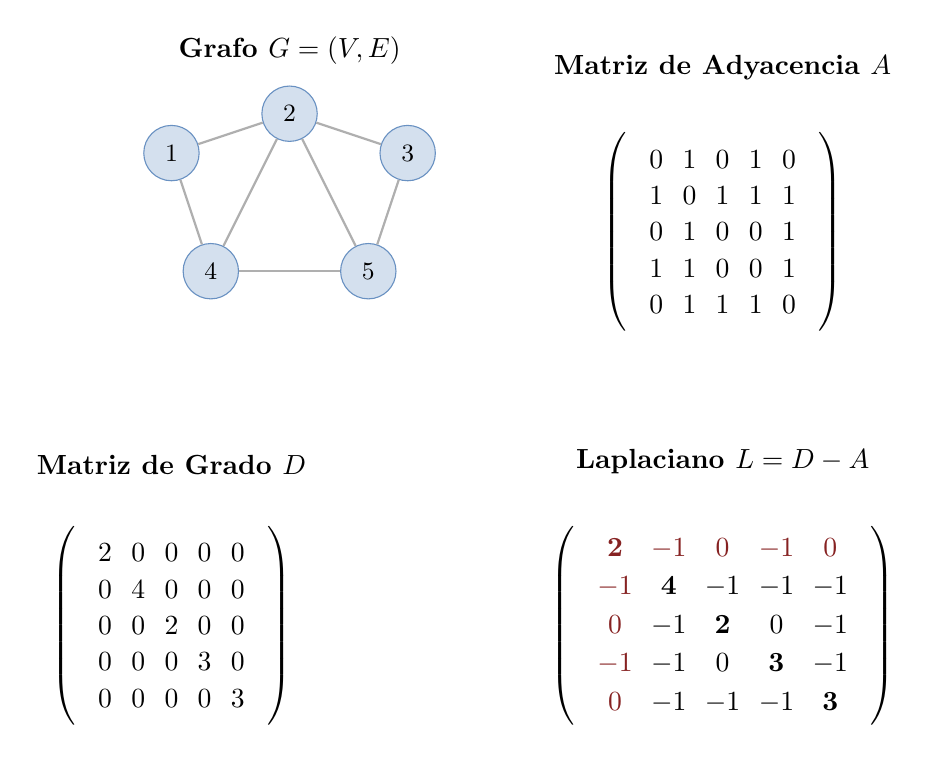
\begin{tikzpicture}[
    vertex/.style={circle, draw=gdlblue!70, fill=gdlblue!20, minimum size=20pt, font=\small},
    edge/.style={thick, draw=gdlgray!70}
]

% === Grafo de ejemplo ===
\begin{scope}[shift={(-4,2)}]
    \node[above, font=\bfseries] at (1.5, 2) {Grafo $G = (V, E)$};

    \node[vertex] (1) at (0,1) {1};
    \node[vertex] (2) at (1.5,1.5) {2};
    \node[vertex] (3) at (3,1) {3};
    \node[vertex] (4) at (0.5,-0.5) {4};
    \node[vertex] (5) at (2.5,-0.5) {5};

    \draw[edge] (1) -- (2);
    \draw[edge] (2) -- (3);
    \draw[edge] (1) -- (4);
    \draw[edge] (2) -- (4);
    \draw[edge] (2) -- (5);
    \draw[edge] (3) -- (5);
    \draw[edge] (4) -- (5);
\end{scope}

% === Matrices ===
\begin{scope}[shift={(3,2)}]
    \node[above, font=\bfseries] at (0, 1.8) {Matriz de Adyacencia $A$};
    \matrix[matrix of math nodes, left delimiter=(, right delimiter=),
            nodes={minimum width=1.2em, minimum height=1.2em}] (A) at (0,0) {
        0 & 1 & 0 & 1 & 0 \\
        1 & 0 & 1 & 1 & 1 \\
        0 & 1 & 0 & 0 & 1 \\
        1 & 1 & 0 & 0 & 1 \\
        0 & 1 & 1 & 1 & 0 \\
    };
\end{scope}

\begin{scope}[shift={(-4,-3)}]
    \node[above, font=\bfseries] at (0, 1.8) {Matriz de Grado $D$};
    \matrix[matrix of math nodes, left delimiter=(, right delimiter=),
            nodes={minimum width=1.2em, minimum height=1.2em}] (D) at (0,0) {
        2 & 0 & 0 & 0 & 0 \\
        0 & 4 & 0 & 0 & 0 \\
        0 & 0 & 2 & 0 & 0 \\
        0 & 0 & 0 & 3 & 0 \\
        0 & 0 & 0 & 0 & 3 \\
    };
\end{scope}

\begin{scope}[shift={(3,-3)}]
    \node[above, font=\bfseries] at (0, 1.8) {Laplaciano $L = D - A$};
    \matrix[matrix of math nodes, left delimiter=(, right delimiter=),
            nodes={minimum width=1.2em, minimum height=1.2em},
            row 1/.style={nodes={text=gdlred!70!black}},
            column 1/.style={nodes={text=gdlred!70!black}}] (L) at (0,0) {
        \mathbf{2} & -1 & 0 & -1 & 0 \\
        -1 & \mathbf{4} & -1 & -1 & -1 \\
        0 & -1 & \mathbf{2} & 0 & -1 \\
        -1 & -1 & 0 & \mathbf{3} & -1 \\
        0 & -1 & -1 & -1 & \mathbf{3} \\
    };
\end{scope}


\end{tikzpicture}
\end{document}
